\documentclass[a4paper,12pt,UTF8,fontset=none]{ctexart}
\usepackage{geometry} % 页面设置
\usepackage{xeCJK}
\usepackage{xcolor} % Color support for listings
\usepackage{graphicx}
\usepackage{amssymb} % For join symbol
\usepackage{amsmath}
\usepackage{listings}
\usepackage{longtable}
\usepackage{booktabs} % 添加booktabs宏包以支持三线表
\usepackage{placeins} 
\usepackage{newtxtext,newtxmath}
\usepackage{fontspec}
\usepackage{titlesec}

% 设置英文主字体为 Times New Roman
\setmainfont{Times New Roman}[Path=D:/Program Files/MiKTeX/fonts/custom/, Extension=.otf]

% 设置英文粗体字体为 Times New Roman Bold
\newfontfamily\enboldfont{Times New Roman Bold}[Path=D:/Program Files/MiKTeX/fonts/custom/, Extension=.otf]

% 设置中文正文字体为宋体
\setCJKmainfont{SimSun}[Path=D:/Program Files/MiKTeX/fonts/custom/, Extension=.ttf]

% 设置中文黑体字体
\setCJKfamilyfont{zhhei}{SimHei}[Path=D:/Program Files/MiKTeX/fonts/custom/, Extension=.ttf]
\newcommand{\heiti}{\CJKfamily{zhhei}}



% 设置标题格式
\titleformat{\section}
  {\heiti\zihao{-3}\enboldfont}{\thesection}{1em}{}
\titleformat{\subsection}
  {\heiti\zihao{4}\enboldfont}{\thesubsection}{1em}{}
\titleformat{\subsubsection}
  {\heiti\zihao{-4}\enboldfont}{\thesubsubsection}{1em}{}



% 设置代码块样式
\lstset{
    basicstyle=\ttfamily,
    columns=fullflexible,
    frame=single,
    breaklines=true,
    postbreak=\mbox{\textcolor{red}{$\hookrightarrow$}\space},
    language=SQL,
    keywordstyle=\color{blue},
    commentstyle=\color{gray},    
    rulecolor=\color{black!30},%边框颜色
    stringstyle=\color{red},
    escapeinside={\%*}{*)},
    showstringspaces=false,
    captionpos=b % 设置标题位置, b表示在底部
}
\geometry{left=2.5cm,right=2.5cm,top=2.5cm,bottom=2.5cm} % 页边距

% 封面设置
\title{SQL数据库系统课后练习}
\author{lanshi}
\date{\today}

\begin{document}

% 制作封面页
\begin{titlepage}
    \centering
    \vspace*{\fill}
    {\LARGE\bfseries 数据库系统原理课程\par}
    \vspace{2cm}
    {\Huge\bfseries SQL课后练习题集\par}
    \vspace{2cm}
    {\Large 烂石\par}
    \vspace{1cm}
    {\large \today \par}
    \vspace{4cm}
    
\includegraphics[width=0.5\textwidth]{images/logo.jpg}
    \vspace*{\fill}
    \thispagestyle{empty} % 封面不显示页码
    \newpage
\end{titlepage}

% 正文内容
\section{ER图相关习题}
\section{关系代数运算相关习题}
例题:现有关系S(S\#,SNAME,AGE,SEX)),C(C\#,CNAME,TEACHER)和SC(S\#,C\#,GRADE),试用表达式表示以下查询语句:
第一个问题:查询至少选修"程军"老师所授全部课程的学生姓名(SNAME);
解析:有三个部分,要查询"程军"老师的全部课程;要查询学生的选课记录,包括学号和课程号;要查询学生的姓名.
至少表示要查询选修了全部课程的学生,即选修了"程军"老师的全部课程的学生.
所以,首先要找到"程军"老师的全部课程,然后找到选修了这些课程的学生,最后找到这些学生的姓名.
这个查询可以分为三个部分:
1.找到"程军"老师的全部课程:\\
\begin{equation}
    \pi_{(C\#(\sigma_(TEACHER='\text{程军}')(C)))}
\end{equation}
2.学生选课记录:\\
\begin{equation}
    \pi_{S\# C\#(SC)}
\end{equation}
3.筛选学生:
\begin{equation}
    {\pi_{S\#,C\#(SC)}}\div{\pi_{(C\#(\sigma_(TEACHER='\text{程军}')(C)}}
\end{equation}
综合以上三个部分,可以得到整个查询的表达式:\\
\begin{equation}
    \pi_{\text{SNAME}} \Big( S \Join \big( \pi_{\text{S\#, C\#}}(SC) \div \pi_{\text{C\#}}( \sigma_{\text{TEACHER='程军'}}(C) ) \big) \Big)
\end{equation}
 
\section{SQL语句}
\subsection{题1:}

1. 设学生课程数据库中有三个关系:

   学生关系 S (S\#, SNAME, AGE, SEX)
    学习关系 SC (S\#, C\#, GRADE)
   课程关系 C (C\#, CNAME)

   其中 S\#, C\#, SNAME, AGE, SEX, GRADE, CNAME 分别表示学号、课程号、姓名、年龄、性别、成绩和课程名。

用 SQL 语句表达以下操作:

1. 检索选修课程名称为 "MATHS" 的学生学号与姓名。
答:\begin{lstlisting}
    SELECT DISTINCT S.S#, S.SNAME
    FROM S
    JOIN SC ON S.S# = SC.S#
    JOIN C ON SC.C# = C.C#
    WHERE C.CNAME = 'MATHS';
\end{lstlisting}
2. 检索至少学习了课程号为 "C1" 和 "C2" 的学生的学号。
\begin{lstlisting}
    SELECT S# FROM SC
    WHERE C# IN("C1","C2")
    GROUP BY S#
    HAVING COUNT (DISTINCT C#)=2
\end{lstlisting}
3. 检索年龄在 18 到 20 之间(含 18 和 20)的女性学生的学号、姓名和年龄。
\begin{lstlisting}
    SELECT S#, SNAME, AGE
    FROM S
    WHERE AGE BETWEEN 18 AND 20
      AND SEX = '女'; 
\end{lstlisting}
4. 检索平均成绩达到 80 的学生学号和平均成绩。
\begin{lstlisting}
    SELECT S#,AVG(GRADE) AS AVG_GRADE
    FROM SC
    GROUP BY S#
    HAVING AVG(GRADE)>=80;
\end{lstlisting}
5. 检索选修了全部课程的学生姓名。
\begin{lstlisting}
    SELECT S.SNAME
    FROM S 
    WHERE NOT EXISTS(
        SELECT C.C#
        FROM C 
        WHERE S# NOT IN(
            SELECT *
            FROM SC
            WHERE S.S#=SC.S#
            AND C.C#=SC.C#
        )
    )
\end{lstlisting}
6. 检索选修了三个课程以上的学生的学号。
\begin{lstlisting}
    SELECT S#
    FROM SC
    GROUP BY S#
    HAVING COUNT(DISTINCT C#) > 3 
\end{lstlisting}
\subsection{题2:学生-课程数据库中包括三个表:}

\begin{itemize}
    \item 学生表:\textbf{Student} (\texttt{Sno}, \texttt{Sname}, \texttt{Sex}, \texttt{Sage}, \texttt{Sdept})
    \item 课程表:\textbf{Course} (\texttt{Cno}, \texttt{Cname}, \texttt{Ccredit})
    \item 学生选课表:\textbf{SC} (\texttt{Sno}, \texttt{Cno}, \texttt{Grade})
\end{itemize}

其中 \texttt{Sno}、\texttt{Sname}、\texttt{Sex}、\texttt{Sage}、\texttt{Sdept}、\texttt{Cno}、\texttt{Cname}、\texttt{Ccredit}、\texttt{Grade} 分别表示学号、姓名、性别、年龄、所在系名、课程号、课程名、学分和成绩。

\textbf{试用 SQL 语言完成下列操作:}

\begin{enumerate}
    \item 查询选修课程包括 “1042” 号学生所学的课程的学生学号。\\
    \begin{lstlisting}
        SELECT DISTINCT Sno
        FROM SC AS X
        WHERE NOT EXISTS (
            SELECT Cno
            FROM SC
            WHERE Sno = '1042'    -- 获取1042学生的所有课程
            AND Cno NOT IN (       -- 检查是否存在1042选修的课程未被当前学生选修
                SELECT Cno
                FROM SC AS Y
                WHERE Y.Sno = X.Sno
            )
        );
    \end{lstlisting}
    \item 创建一个计算系学生信息视图 \textbf{CS\_VIEW},包括 \texttt{Sno} 学号、\texttt{Sname} 姓名、\texttt{Sex} 性别。
    \begin{lstlisting}
        CREATE VIEW CS_VIEW AS
        SELECT Sno,Sname,Sex
        FROM Student
        WHERE Sdept='计算系'
    \end{lstlisting}
    \item 通过上面第 2 题创建的视图修改数据,把王平的名字改为王慧平。
    \begin{lstlisting}
        UPDATE CS_VIEW
        SET Sname='王慧平'
        WHERE Sname='王平'
    \end{lstlisting}
    \item 创建一选修数据库课程信息的视图,视图名称为 \textbf{datascore\_view},包含学号、姓名、成绩。
    \begin{lstlisting}
        CREATE VIEW datascore_view AS
        SELECT Student.Sno, Sname, Grade
        FROM Student
        JOIN SC ON Student.Sno = SC.Sno
        JOIN Course ON SC.Cno = Course.Cno
        WHERE Course.Cname = '数据库';
    \end{lstlisting}
\end{enumerate}

\section{关系模式}
\subsection*{题1:已知学生关系模式如下:}
\par 关系模式 $S(Sno, Sname, SD, Sdname, Course, Grade)$

其中:\par  
$Sno$ 学号,  \par
$Sname$ 姓名,  \par
$SD$ 系名,  \par
$Sdname$ 系主任名,\par
$Course$ 课程,  \par
$Grade$ 成绩。  

\begin{enumerate}
  \item 写出关系模式 $S$ 的基本函数依赖和主码。
  \begin{center}
  $Sno \rightarrow Sname $\\
  $Sno \rightarrow Course$\\
  $(Sno,Course) \rightarrow Grade$\\
  $Sno \rightarrow SD$\\
  $SD \rightarrow Sdname$
  \par 主码为(Sno,Course)
  \end{center}
  \item 原关系模式 $S$ 为几范式?为什么?分解成高一级范式,并说明为什么?
  原关系模式为1NF,Grade对主码存在完全依赖;
  其他非主码候选健对主码存在部分依赖.
  2NF如下所示:\par
  \begin{center}
    
  $S1(Sno,Sname,SD,Sdname)$\\
  $S2(Sno,Course,Grade)$\\
  \end{center}
  \item 将关系模式分解成 3NF,并说明为什么。
  S1存在传递依赖,还可以继续分解
  3NF如下所示:\par
  \begin{center}
    
  $S11(Sno,Sname,SD)$\\
  $S12(SD,Sdname)$\\
  $S2(Sno,Course,Grade)$
  \end{center}
\end{enumerate}
\subsection*{题2:设有如下关系 R}
\FloatBarrier
\begin{table}[htbp]
    \centering
    \caption{关系 R}
    \vskip 2mm
    \begin{tabular}{ccc}
        \toprule % 顶部粗线
        \textbf{课程名} & \textbf{教师名} & \textbf{教师地址} \\ 
        \midrule % 中间细线
        C1 & 马千里 & D1 \\ 
        C2 & 于得水 & D1 \\ 
        C3 & 余快 & D2 \\ 
        C4 & 于得水 & D1 \\ 
        \bottomrule % 底部粗线
    \end{tabular}
\end{table}

\begin{enumerate}
    \item 它为几范式?为什么?
    \par 2NF,存在传递依赖,\\$\text{课程名} \rightarrow \text{教师名}$\\
    $\text{教师名} \rightarrow \text{教师地址}$\\
    存在$\text{课程名} \rightarrow \text{教师地址}$的传递依赖;但又不存在部分函数依赖.
    属于2NF
    \item 是否存在删除操作异常?若存在,则说明是在什么情况下发生的?
    \par 存在,当删除课程名时,可能某些信息会全部丢失
    \item 将它分解为高一级范式,分解后的关系是如何解决分解前可能存在的删除操作问题的?
    \par 转为3NF,消除传递依赖,分解原表为R1,R2
    \begin{table}[htbp]
        \centering
        \caption{关系 R1}
        \vskip 2mm
        \begin{tabular}{ccc}
            \toprule % 顶部粗线
            \textbf{课程名} & \textbf{教师名}  \\ 
            \midrule % 中间细线
            C1 & 马千里  \\ 
            C2 & 于得水  \\ 
            C3 & 余快  \\ 
            C4 & 于得水 \\ 
            \bottomrule % 底部粗线
        \end{tabular}
    \end{table}
    \begin{table}[htbp]
        \centering
        \caption{关系 R2}
        \vskip 2mm
        \begin{tabular}{ccc}
            \toprule % 顶部粗线
             \textbf{教师名} & \textbf{教师地址} \\ 
            \midrule % 中间细线
             马千里 & D1 \\ 
             于得水 & D1 \\ 
             余快 & D2 \\ 
            \bottomrule % 底部粗线
        \end{tabular}
    \end{table}
\end{enumerate}
\FloatBarrier
\subsection*{题3. 设某商业集团数据库中有一关系模式 R 如下:}

   R (商店编号, 商品编号, 数量, 部门编号, 负责人)

   如果规定:(1) 每个商店的每种商品只能在一个部门销售;(2) 每个商店的每个部门只有一个负责人;(3) 每个商店的每种商品只有一个库存数量。

   试回答下列问题:

   (1) 根据上述规定,写出关系模式 R 的基本函数依赖;
   \begin{center}
   $\text{部门编号} \rightarrow \text{负责人}$\\
   $\text{商品编号} \rightarrow \text{数量}$\\
   $(\text{商店编号,商品编号}) \rightarrow \text{部门编号}$\\
   \end{center}

   (2) 找出关系模式 R 的候选码;
   \par (商店编号,商品编号)

   (3) 试问关系模式 R 最高已经达到第几范式?为什么?
   \par 2NF,存在$\mbox{(商店编号,商品编号)} \rightarrow \mbox{负责人}$的传递依赖.

   (4) 如果 R 不属于 3NF,请将 R 分解成 3NF 模式集。
   \par R1(商店编号,商品编号,部门编号,数量)

   R2(商品编号,商店编号,负责人)
\section{实体关系模型设计}

   \subsection*{题1:设有如下实体:学生、学号、姓名、性别、年龄、选修课程名;教师:教师号、姓名、性别、职称、讲授课程编号;课程:编号、课程名、开课单位、任课教师号。}
   
   上述实体中存在如下关联:
   
   \begin{enumerate}
       \item 一个学生可选择多门课程,一门课程可由多个学生选择;
       \item 一个教师可讲授多门课程,一门课程可由多个教师讲授;
       \item 一个单位有多个教师,一个教师只能属于一个单位。
   \end{enumerate}
   
   试完成如下任务:
   
   \begin{enumerate}
       \item 分别设计学生信息和教师信息的 E-R 图;
       \item 将上述设计完成的 E-R 图合并成一个全局 E-R 图;
       \par 题1,题2如图所示\ref{图5-1}
       \FloatBarrier
       \begin{figure}[htbp]
        \centering
        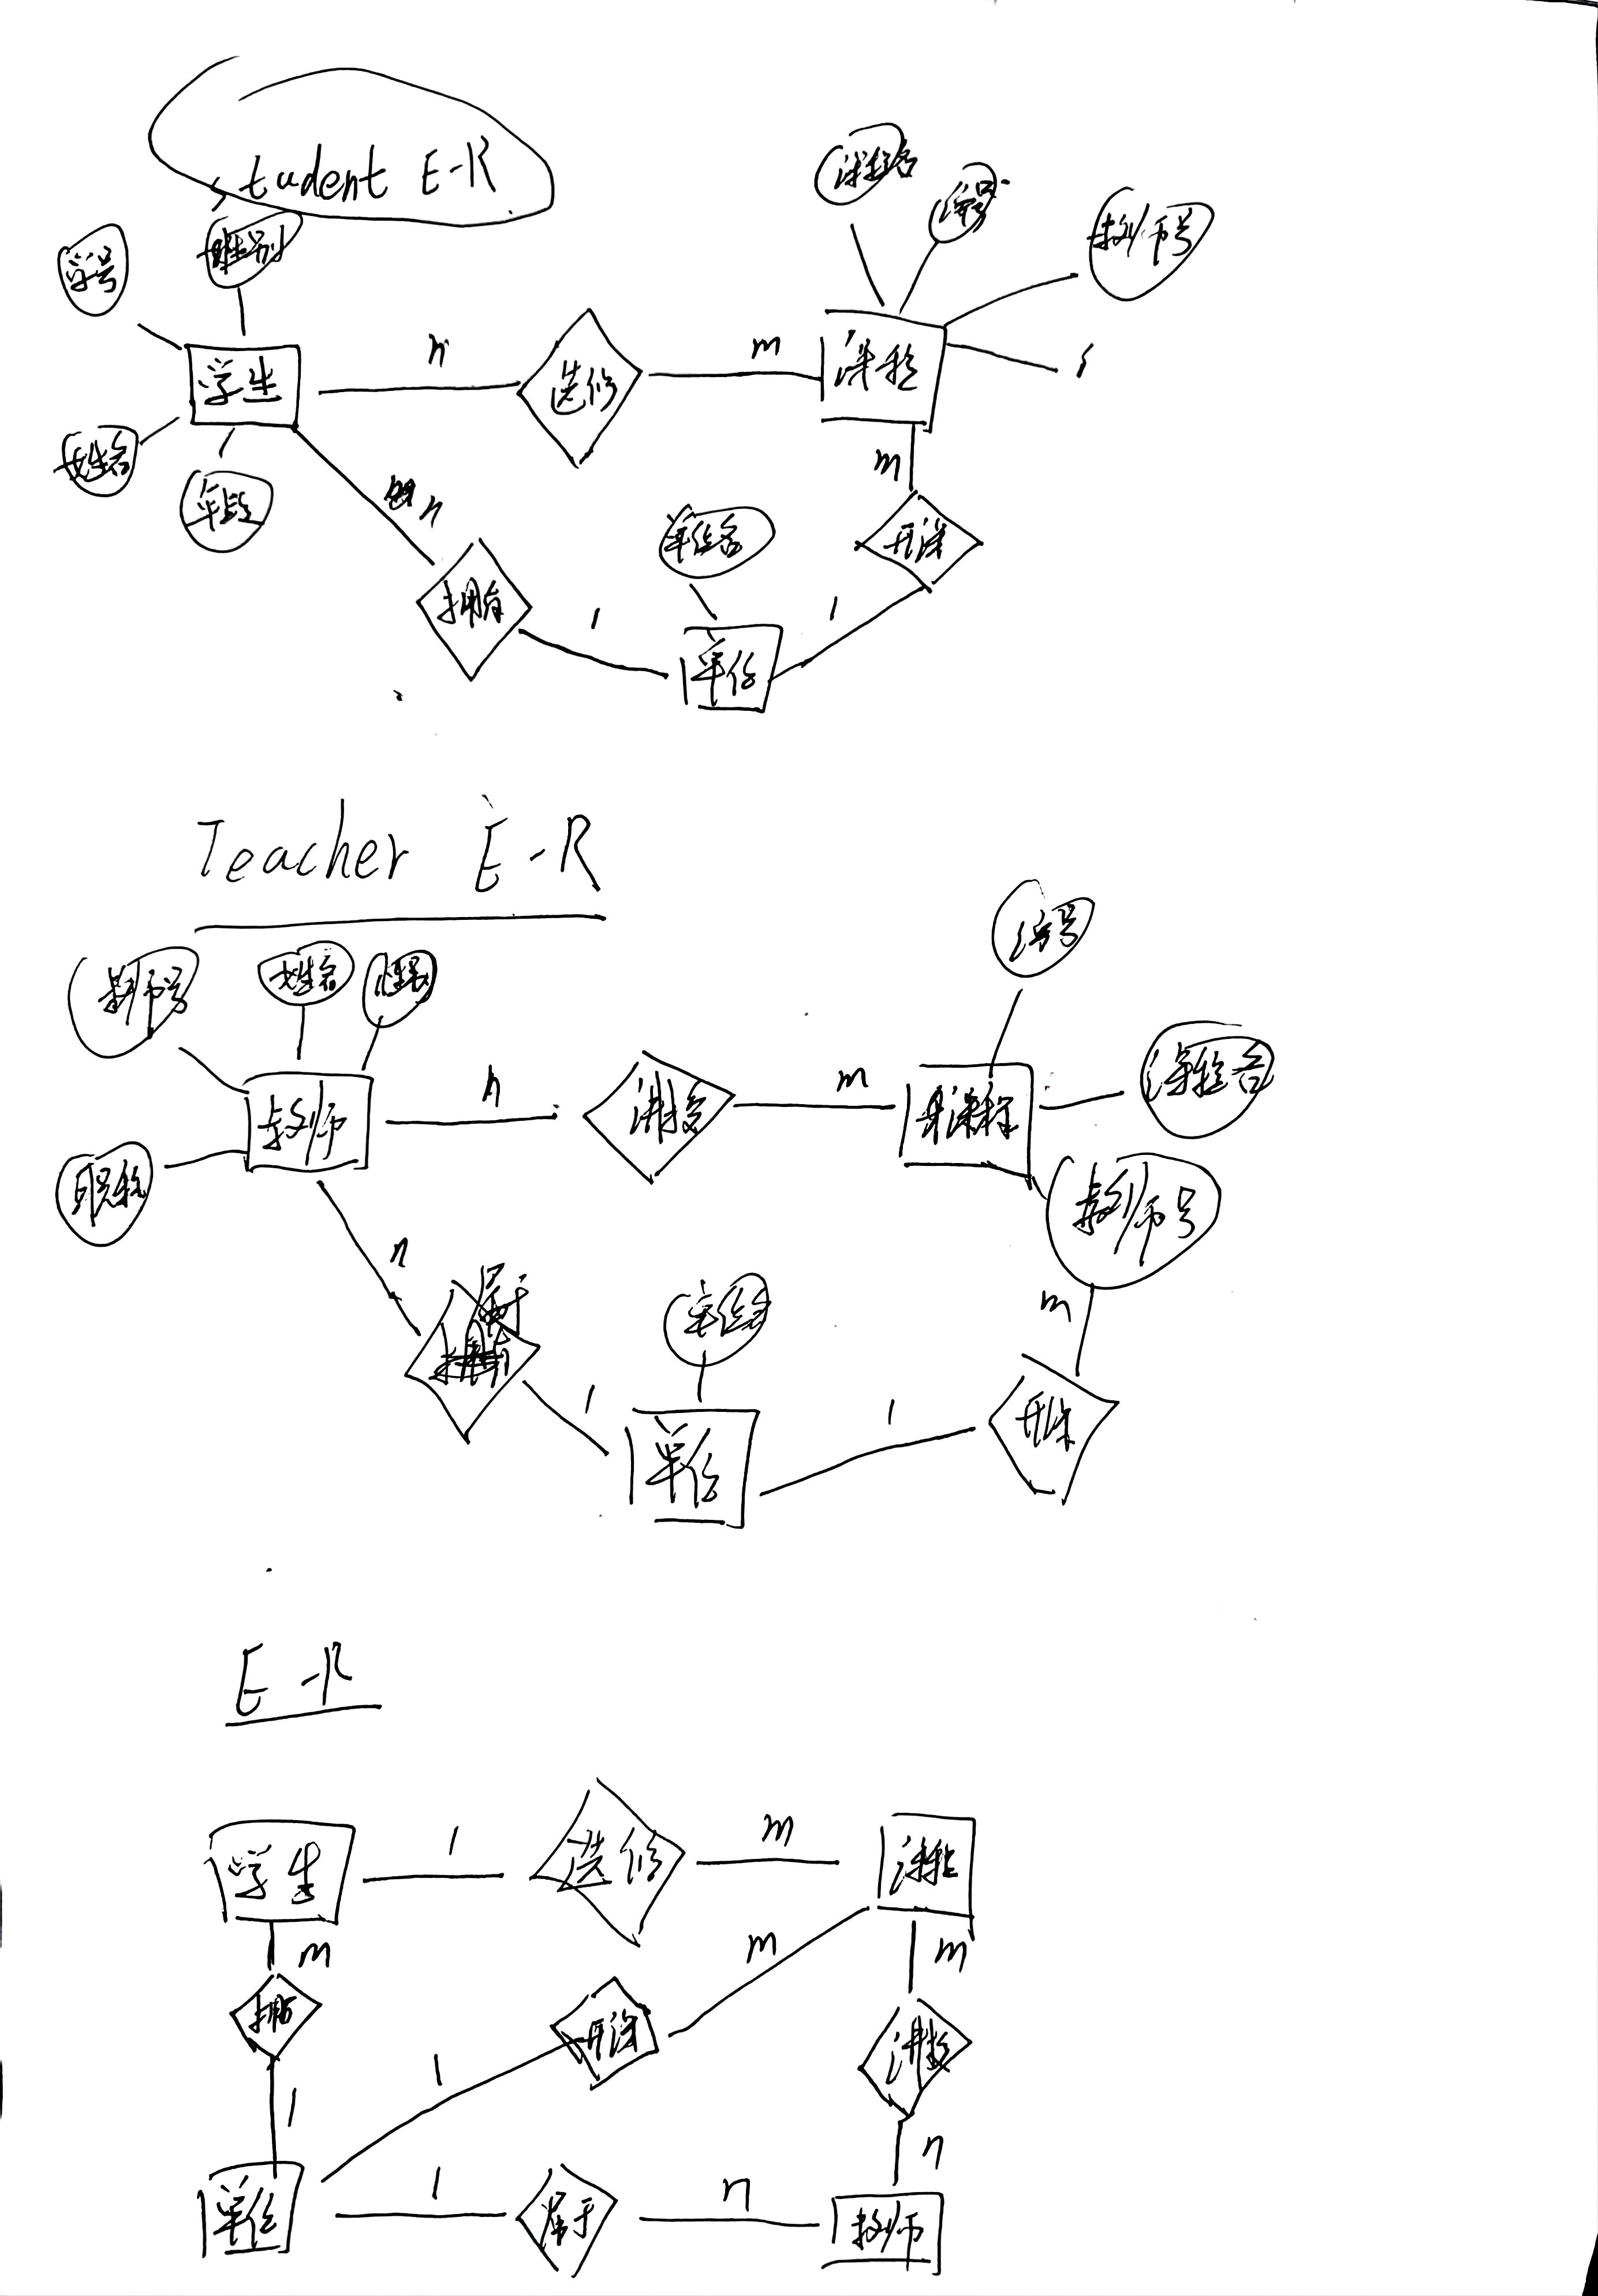
\includegraphics[width=0.8\textwidth]{./images/题1-E-R图.jpg}
        \caption{题目1的一二小问E-R图}
        \label{图5-1}
    \end{figure}
    \FloatBarrier
       \item 将该全局 E-R 图转换为对应的数据库逻辑结构。
       \begin{lstlisting}
        CREATE TABLE Student(
            sno VARCHAR(20) PRIMARY KEY,
            sname VARCHAR(50),
            sex CHAR(1),
            age INT
        );
       \end{lstlisting}
   \end{enumerate}
\end{document}